\begin{figure}[h]
\centering
\begin{subfigure}[t]{0.45\textwidth}
\centering
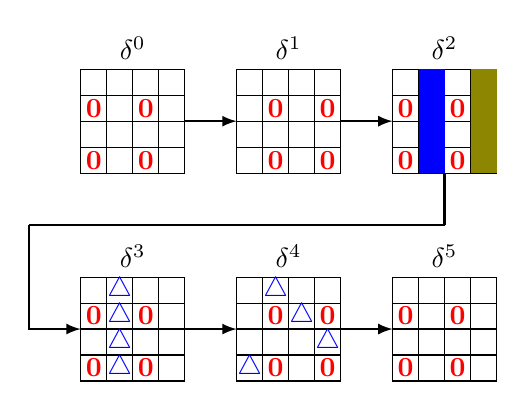
\begin{tikzpicture}[scale=.33]
\foreach \i in {0,...,2}{
	\foreach \j in {0,...,3}{
		\foreach \k in {0,...,3}{
			\draw (0 + \k + 6*\i,0 + \j) rectangle (1 + \k + 6*\i,1 + \j);
			\draw (0 + \k + 6*\i,0 + \j - 8) rectangle (1 + \k + 6*\i,1 + \j - 8);
		}
	}
}
\draw[->,>=latex,thick] (4,2) -- (6,2) node[above,midway] {$\shiftR$};
\draw[->,>=latex,thick] (10,2) -- (12,2) node[above,midway] {$\mixC$};

\draw[thick] (14,0) -- (14, -2);
\draw[thick] (14,-2) -- (-2,-2) node[above,midway] {$\subW$};
\draw[->,>=latex,thick] (-2,-2) -- (-2,-6) -- (0,-6);

\draw[->,>=latex,thick] (4,-6) -- (6,-6) node[above,midway] {$\shiftR$};
\draw[->,>=latex,thick] (10,-6) -- (12,-6) node[above,midway] {$\mixC$};

\draw (2,4) node[above] {$\delta^0$};
\draw (8,4) node[above] {$\delta^1$};
\draw (14,4) node[above] {$\delta^2$};
\draw (2,-4) node[above] {$\delta^3$};
\draw (8,-4) node[above] {$\delta^4$};
\draw (14,-4) node[above] {$\delta^5$};

%zero conditions
\foreach \j in {0,7,12}{
\foreach \i in {0,8}{
\draw (.5 + \j,.5 - \i) node {$\color{red}{\mathbf{0}}$};
\draw (2.5 + \j,.5 - \i) node {$\color{red}{\mathbf{0}}$};
\draw (.5 + \j,2.5 - \i) node {$\color{red}{\mathbf{0}}$};
\draw (2.5 + \j,2.5 - \i) node {$\color{red}{\mathbf{0}}$};
}

}
%olive and blue conditions
\foreach \i in {0,1,2,3}{
\fill[blue] (13,\i) rectangle (14,\i + 1);
\fill[olive] (15,\i) rectangle (16,\i + 1);
\draw (1.5,-7.5+\i) node {$\color{blue}{\mathbf{\triangle}}$};
\draw (3.5,-7.5+\i) node {$\color{olive}{\mathbf{\square}}$};
}
\draw (7.5,-4.5) node {$\color{blue}{\mathbf{\triangle}}$};
\draw (8.5,-5.5) node {$\color{blue}{\mathbf{\triangle}}$};
\draw (9.5,-6.5) node {$\color{blue}{\mathbf{\triangle}}$};
\draw (6.5,-7.5) node {$\color{blue}{\mathbf{\triangle}}$};

\draw (9.5,-4.5) node {$\color{olive}{\mathbf{\square}}$};
\draw (6.5,-5.5) node {$\color{olive}{\mathbf{\square}}$};
\draw (7.5,-6.5) node {$\color{olive}{\mathbf{\square}}$};
\draw (8.5,-7.5) node {$\color{olive}{\mathbf{\square}}$};



\end{tikzpicture}
\caption{\label{fig:difftrail}Conditions.}

\end{subfigure}
\hfill
\begin{subfigure}[t]{0.45\textwidth}
\centering
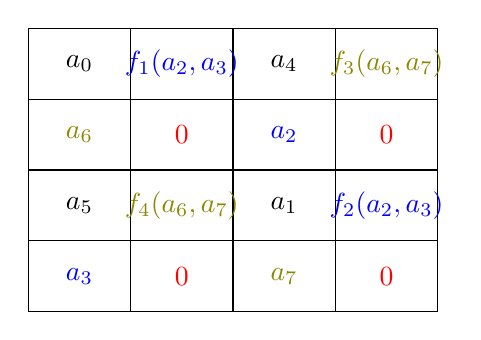
\begin{tikzpicture}[xscale=1.3, yscale=0.9]
\foreach \i in {0,1,2,3}{
	\foreach \j in {0,1,2,3}{
		\draw (\i,\j) rectangle (\i + 1, \j + 1);
	}
}
\draw (.5,3.5) node {$a_0$};
\draw (1.5,3.5) node {$\color{blue}{f_1(a_2,a_3)}$};
\draw (2.5,3.5) node {$a_4$};
\draw (3.5,3.5) node {$\color{olive}{f_3(a_6,a_7)}$};

\draw (.5,2.5) node {$\color{olive}{a_6}$};
\draw (1.5,2.5) node {$\color{red}{0}$};
\draw (2.5,2.5) node {$\color{blue}{a_2}$};
\draw (3.5,2.5) node {$\color{red}{0}$};

\draw (.5,1.5) node {$a_5$};
\draw (1.5,1.5) node {$\color{olive}{f_4(a_6,a_7)}$};
\draw (2.5,1.5) node {$a_1$};
\draw (3.5,1.5) node {$\color{blue}{f_2(a_2,a_3)}$};

\draw (.5,.5) node {$\color{blue}{a_3}$};
\draw (1.5,.5) node {$\color{red}{0}$};
\draw (2.5,.5) node {$\color{olive}{a_7}$};
\draw (3.5,.5) node {$\color{red}{0}$};
\end{tikzpicture}
\caption{\label{fig:solutiondelta4}Formal conditions for $\delta^4$.}


\end{subfigure}
\caption{\label{fig:proofindependent}The conditions to have $F^{(3)}(X,K_0,K_1) - F^{(3)}(X+\delta,K_0,K_1) = 0$.}
\end{figure}

